Bevor die Subscription erstellt bzw. vom Smartphone angefordert wird, herrscht folgende Ausgangssituation. Vor der Inbetriebnahme des Verleihdienstes müssen Smartphone, Back End und Mikrocontroller jeweils über ein individuelles Zertifikat (nach X.509-Standard) und dessen privaten Schlüssel verfügen. Die Zertifikate wurden jeweils von der Zertifizierungsstelle ausgestellt. Zudem kennt auch jede der drei Parteien (Smartphone, Back End, Mikrocontroller) das Root-Zertifikat (das Zertifikat der Zertifizierungsstelle), um damit die anderen Parteien authentifizieren zu können. Außerdem benötigt das Back End ein weiteres Zertifikat mit zugehörigem privaten Schlüssel, das Subscription-Zertifikat genannt wird.
\\\\
Nun möchte ein Nutzer mit der Smartphone-Anwendung (App) ein Fahrzeug ausleihen. Dafür sollte das Fahrzeug signalisieren, dass es für einen Ausleihvorgang zur Verfügung steht. Ab diesen Punkt ist der weitere Verlauf des Ausleihprozesses in Abb. \ref{fig: verlauf ausleihprozess} dargestellt.
\begin{figure}[H]
    \centering
    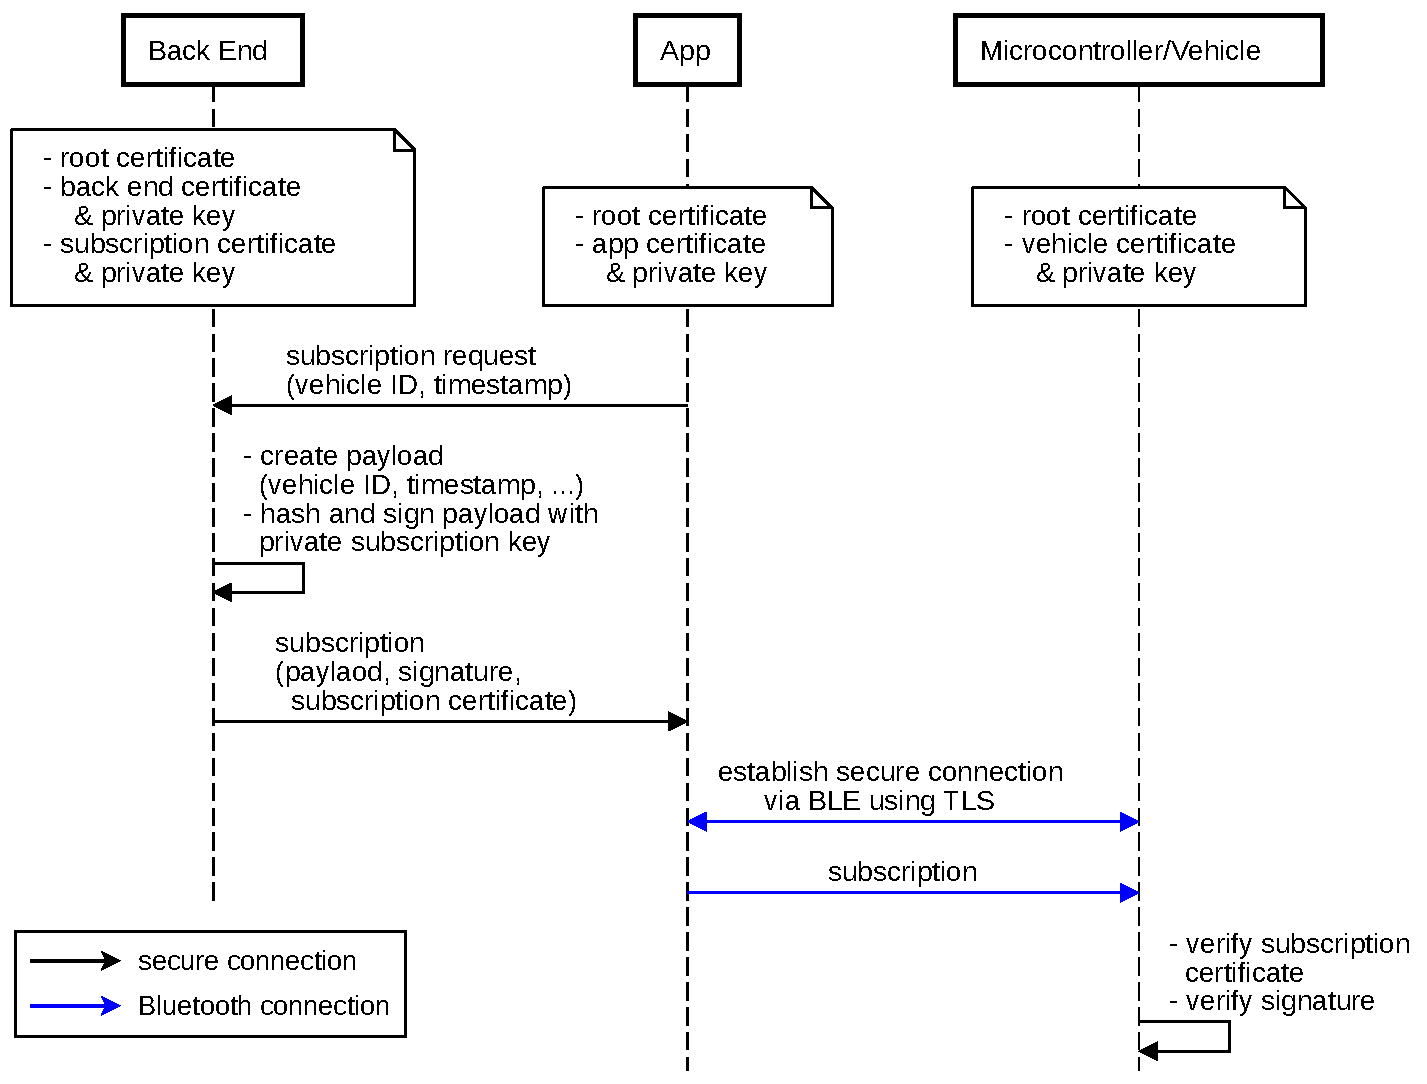
\includegraphics[width=1\textwidth]{graphics/verlauf_ausleihprozess.pdf}
    \caption[Verlauf des Ausleihprozzeses]{Verlauf des Ausleihprozzeses}
    \label{fig: verlauf ausleihprozess}
\end{figure}
Zu Beginn muss die App die Identität und Bluetooth-Adresse des Fahrzeugs feststellen (z.B. über einen Quick Response Code, kurz QR-Code). Die App baut eine sichere Verbindung zum Back End auf und verlangt nach einer Subscription. Dabei sendet sie die Identität des Fahrzeugs, einen aktuellen Zeitstempel und evtl. weitere Informationen (z.B. bzgl. des Bezahlmodells). Das Back End fügt zu diesen Informationen evtl. noch weitere hinzu (z.B. bzgl. des Bezahlmodells) und formt daraus den "`Payload"'. Danach wird der Hashwert des Payloads gebildet und mit dem privaten Schlüssel signiert. Die Subscription setzt sich nun entsprechend Abb. \ref{fig: aufbau subscription} zusammen.
\begin{figure}[H]
    \centering
    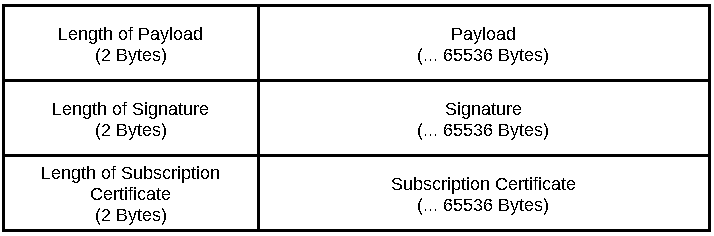
\includegraphics[width=0.9\textwidth]{graphics/aufbau_subscription.pdf}
    \caption[Aufbau der Subscription]{Aufbau der Subscription}
    \label{fig: aufbau subscription}
\end{figure}
Das erste Längenfeld gibt die Länge des darauffolgenden Payloads an. Das zweite Längenfeld gibt die Länge der Signatur an, worauf die Signatur folgt. Das letzte Längenfeld steht für die Länge des Subscription-Zertifikats und ist gefolgt vom Subscription-Zertifikat. Schließlich überträgt das Back End die Subscription an die App und trennt die Verbindung.
\\\\
Entsprechend der Sektion \ref{sec: infra verbindungsaufbau} verbindet sich die App über BLE mit dem Fahrzeug und stellt mittels TLS eine sichere Verbindung her. Daraufhin beendet das Fahrzeug das Advertising. Anschließend sendet die App die Subscription an das Fahrzeug. Zuerst verifziert das Fahrzeug das Subscription-Zertifikat, indem es dessen Signatur mit dem Root-Zertifikat prüft. Danach verifiziert es die Signatur des Payloads mit der gleichen Hash-Funktion, die zur Erstellung der Signatur genutzt wurde, und dem öffentlichen Schlüssel des Subscription-Zertifikats. Sind die Verifikationen erfolgreich, konnte das Fahrzeug sicherstellen, dass die Subscription vom Back End erstellt wurde. Nun müssen noch die Inhalte des Payloads geprüft werden. Demnach muss die angegebene Identität mit der des Fahrzeugs übereinstimmen und der Zeitstempel aktuell sein. Wurden weitere Informationen angegeben, sollte deren Plausibilität geprüft deren Informationsgehalt verarbeitet werden. Somit ist der erste Teil des Ausleihprozesses abgeschlossen. Sollte eine der Verifikationen fehlschlagen sowohl bei der Prüfung der Subscription als auch vorher auf Ebene von TLS, wird die Verbindung abgebrochen.